\chapter{Conti 3D}

Si consideri la generica mappa che passa dalla slice reale a quella di riferimento.

\begin{center}
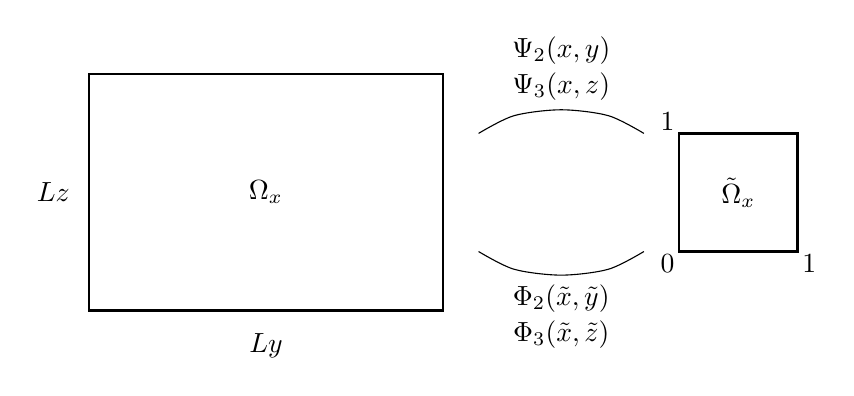
\begin{tikzpicture}
[scale=1.5]

\draw [thick] (0,0) rectangle (3,2);
\node at (1.5,1) {$\Omega_x$};
\node at (1.5, -0.3) {$Ly$};
\node at (-0.3,1) {$Lz$};

\draw [thick] (5,0.5) rectangle (6,1.5);
\node at (5.5,1)  {$\tilde{\Omega}_{x}$};
\node at(6.1,0.4)  {$1$};
\node at(4.9,1.6) {$1$};
\node at(4.9,0.4) {$0$};

\draw plot [->,smooth] coordinates {(3.3,1.5) (3.6,1.65) (4,1.7) (4.4,1.65) (4.7,1.5)};

\node at (4,2.2) {$\Psi_2(x,y)$};
\node at (4,1.9) {$\Psi_3(x,z)$};

\draw plot [<-,smooth] coordinates {(3.3,0.5) (3.6,0.35) (4,0.3) (4.4,0.35) (4.7,0.5)};
\node at (4,0.1) {$\Phi_2(\tilde{x},\tilde{y})$};
\node at (4,-0.2) {$\Phi_3(\tilde{x},\tilde{z})$};


\end{tikzpicture}
\end{center}

Consideriamo una mappa della seguente forma:

\begin{equation}
\label{eq: mappa generica}
\begin{array}{l l}
&\Psi_1 = x; \\
\vect{\Psi}(x,y,z) := \Bigg\{ &\Psi_2 = \Psi_2(x,y); \\
&\Psi_3 = \Psi_3(x,z); \\
\end{array}
\end{equation} 

Lo Jacobiano prodotto sar\`a della forma seguente (si noti che $x = \tilde{x}$):

\begin{equation}
\begin{array}{c}
J_{\vect{\Psi}}(x,y,z) := \left[ \begin{array}{c c c}
1&0&0\\
\partial_x\Psi_2(x,y)&\partial_y\Psi_2(x,y)&0\\
\partial_x\Psi_3(x,z)&0&\partial_z\Psi_3(x,z)
\end{array}
\right]

\end{array}
\end{equation}


Lo spazio ridotto viene costruito sul dominio di riferimento, ovvero il parallelepipedo di sezione $(0,1)\times(0,1)$ e lunghezza pari alla lunghezza reale $L_x$.

\begin{equation}
\label{eq: spazio ridotto}
V_m := \left\{ v_m(x,y,z) = \sum_{k=1}^m v_k(\Psi_1(x))\varphi_k(\Psi_2(x,y),\Psi_3(x,z)): v_k \in V_{\tilde{\Omega}_{1D}} \right\}
\end{equation}

Le $\varphi_k(\Psi_2(x,y),\Psi_3(x,z)$ sono invece le basi modali costruite sulla slice di riferimento. Ricordiamo la formulazione debole del problema in analisi:

\begin{multline}
\int_\Omega\left(\mu\nabla u_m\nabla v_m + \vect{b}\nabla u_mv_m+\sigma u_mv_m\right)\,d\Omega
=\int_\Omega fv \,dxdy
\end{multline}

Consideriamo la seguente espressione per $u_m$, dove si \`e definito $\vect{\Psi_2}(\vect{x}):=(\Psi_2(x,y),\Psi_3(x,z))$,

\begin{equation}
u_m(x,y,z) := \sum_{j=1}^m u_j(x)\varphi_j(\vect{\Psi_2}(\vect{x}))
\end{equation}

Procediamo con i calcoli sapendo che:

\begin{equation}
\nabla(u_j(x)\varphi_j(\vect{\Psi_2}(\vect{x})) = \left[ 
\begin{array}{c}
u_j'(x)\varphi_j(\vect{\Psi_2}(\vect{x})) + u_j(x)\tilde{\nabla}\varphi_j\cdot \partial_x \vect{\Psi_2}) \\
u_j(x)\tilde{\nabla}\varphi_j\cdot \partial_y \vect{\Psi_2})\\
u_j(x)\tilde{\nabla}\varphi_j\cdot \partial_z \vect{\Psi_2})
\end{array}
\right]
\end{equation}


\begin{equation}
\begin{array}{c c}
\tilde{\nabla}\varphi_j := \left[
\begin{array}{c}
\partial_{\tilde{y}}\varphi_j \\
\partial_{\tilde{z}}\varphi_j
\end{array}
\right]
&
\partial_i\vect{\Psi_2} := \left[
\begin{array}{c}
\partial_i\Psi_2 \\
\partial_i\Psi_3
\end{array}
\right]
\end{array}
\end{equation}

Riscriviamo quindi la formulazione come segue:

\begin{equation}
\label{eq: formulazione 1}
\begin{array}{l}
\int_\Omega \mu(\vect{x})
(\\
u_j'(x)\vartheta'(x)\varphi_j(\vect{\Psi_2}(\vect{x})\varphi_k(\vect{\Psi_2}) \\

+ u_j'(x)\vartheta(x)\varphi_j(\vect{\Psi_2}(\vect{x})[\tilde{\nabla}\varphi_k(\vect{\Psi_2}) \cdot \partial_x\vect{\Psi_2}]\\

+u_j(x)\vartheta'(x)[\tilde{\nabla}\varphi_j(\vect{\Psi_2}(\vect{x})\cdot \partial_x\vect{\Psi_2}]\varphi_k(\vect{\Psi_2}) \\

+u_j(x)\vartheta(x)[\tilde{\nabla}\varphi_j(\vect{\Psi_2}(\vect{x})\cdot \partial_x\vect{\Psi_2}][\tilde{\nabla}\varphi_k(\vect{\Psi_2})\cdot \partial_x\vect{\Psi_2}] \\

+u_j(x)\vartheta(x)[\tilde{\nabla}\varphi_j(\vect{\Psi_2}(\vect{x})\cdot \partial_y\vect{\Psi_2}][\tilde{\nabla}\varphi_k(\vect{\Psi_2})\cdot \partial_y\vect{\Psi_2}] \\

+u_j(x)\vartheta(x)[\tilde{\nabla}\varphi_j(\vect{\Psi_2}(\vect{x})\cdot \partial_z\vect{\Psi_2}][\tilde{\nabla}\varphi_k(\vect{\Psi_2})\cdot \partial_z\vect{\Psi_2}] \\
 )\,d\Omega \\
 
 + \int_\Omega \\
 b_1(\vect{x})\vartheta(x)\varphi_k(\vect{\Psi_2})
 (u_j'(x)\varphi_j(\vect{\Psi_2})+u_j(x)[\tilde{\nabla}\varphi_j(\vect{\Psi_2}(\vect{x})\cdot \partial_x\vect{\Psi_2}]) \\
 + b_2(\vect{x})\vartheta(x)\varphi_k(\vect{\Psi_2})
u_j(x)[\tilde{\nabla}\varphi_j(\vect{\Psi_2}(\vect{x})\cdot \partial_y\vect{\Psi_2}] \\
+
b_3(\vect{x})\vartheta(x)\varphi_k(\vect{\Psi_2})
u_j(x)[\tilde{\nabla}\varphi_j(\vect{\Psi_2}(\vect{x})\cdot \partial_z\vect{\Psi_2}] \\
\,d\Omega\\
+
\int_\Omega \sigma(\vect{x})u_j(x)\vartheta(x)\varphi_j(\vect{\Psi_2})
\varphi_k(\vect{\Psi_2})
\,d\Omega\\
= \int_\Omega f(\vect{x})\vartheta(x)\varphi_k(\vect{\Psi_2})
\,d\Omega
\end{array}
\end{equation}